\documentclass[]{article}
\usepackage{fontspec} % compile w/XeLaTeX
\usepackage{lmodern}
\usepackage{setspace} % ability to set the line spacing
\usepackage[fontsize=13]{scrextend}
\usepackage[a4paper, tmargin=0.79in, left=1.38in, right=1.38in,bmargin=1.18in]{geometry}
\usepackage{fancyhdr, graphicx, lastpage}
\usepackage{amsmath}
\usepackage{bm}
\usepackage{caption}
\usepackage{subcaption}
\usepackage{ragged2e}
\usepackage{graphicx}
\usepackage{float}
\usepackage{matlab-prettifier}
\usepackage{pdfpages}
\usepackage{hyperref}
\usepackage{cleveref}
\usepackage{verbatim}
\usepackage{chngcntr}
\usepackage{upgreek}
\usepackage{url}
\usepackage[title]{appendix}
\usepackage[sorting=none, backend=biber, style=ieee]{biblatex} 
\addbibresource{Thesis.bib}
\setcounter{secnumdepth}{4}
\usepackage[labelsep=period]{caption}
\captionsetup[table]{name=Table}
\renewcommand{\thetable}{\Roman{table}}
\makeatletter
\def\input@path{"./MATLAB Software"}
\makeatother
\graphicspath{{./figures/}}
\graphicspath{{./images/}}
\allowdisplaybreaks
\usepackage[parfill]{parskip} %Change indents to line breaks between paragraphs
\usepackage[acronym, style=super, nonumberlist]{glossaries}
\emergencystretch=1em % Used to make badness error for bibliography go away

\newacronym{CM}{CM}{Condition Monitoring}
\newacronym{PM}{PM}{Predictive Maintenance}
\newacronym{RMS}{RMS}{Root Mean Square}
\newacronym{SNR}{SNR}{Signal to Noise Ratio}
\newacronym{THD}{THD}{Total Harmonic Distortion}
\newacronym{SINAD}{SINAD}{Signal-to-noise and Distortion Ratio}
\newacronym{TSS}{TSS}{Total Sum of Squares}
\newacronym{SSR}{SSR}{Sum of Squared Regression}
\newacronym{PCA}{PCA}{Principal Component Analysis}
\newacronym{NRMSE}{NRMSE}{Normalized Root Mean Square Error}
\newacronym{FFT}{FFT}{Fast Fourier Transform}
\makenoidxglossaries

\newcommand{\appendixpagenumbering}{
  \break
  \pagenumbering{arabic}
  \renewcommand{\thepage}{\thesection\arabic{page}}
}

\begin{document}
\setmainfont{Perpetua}
\setstretch{1.15}

\includepdf[]{Coverpage_Barron.pdf}
\setglossarystyle{index}
\newpage
\thispagestyle{empty}
\mbox{}
\newpage
\pagenumbering{roman}

\section*{Acknowledgments}
I would like to express deep gratitude to my supervisors, Daniel Rönnow and Oscar Bautista Gonzalez, for their time, guidance and support. To the University of Gävle I am extremely appreciative for opportunity to complete a Masters Program in Electronics and Automation available as distance education. This is ideal for full time working professionals and is the only course of it's kind in Sweden. Special thanks to thank Alleima for providing the data to analyze for this Thesis, without which it would not have been possible. Finally, I would also like to acknowledge the fact that I am undertaking this study for no personal cost thanks to free education offered by the Swedish Government. More countries should consider offering free education. Knowledge is power.
\newpage

\section*{Abstract}
% Some general comment on the reasons for the project
The availability of industrial machinery is crucial to any business operating in the manufacturing sector. Mechanical failures halt production and unplanned downtime can be disruptive and costly. Small failures can escalate to more serious failures which exponentially increases downtime and repair costs. Identifying a degradation condition before reaching catastrophic failure is key to maintaining machine availability. On the other hand, it's undesirable to expend resources performing unrequited maintenance. For these reasons a large field of academic work is dedicated to analyzing the health of a machine, predicting it's remaining life and in turn preventing failures.

% What the project is about
This thesis analyses data from a tube straightening machine used in the steel industry with the end goal of implementing a condition monitoring strategy. The data comes from a real world application provided by a multinational manufacturer of steel products. It was obtained using the existing sensors and data acquisition system. The project serves as a study of the existing infrastructure (available sensors) and it's suitability for implementing a condition monitoring strategy. The work is the first step in a larger study and does not attempt to perform any implementation or fault identification. In a broad sense the aim of the project is to identify relationships and patterns in the data that could be varying with time as the machine degrades.

% Outling of project steps
The data consists of twelve channels taken over a two week duration. It is prepossessed to isolate periods where the machine is operating and separated into cycles. Each of these is then further processed to extract time and frequency domain features. The features within each channel are compared with each other using the $R_2$ coefficient of determination to find combinations that are correlated. A semi automated process is used to select the feature combinations. The same process is performed between signals for each feature. 

% The conclusions of the project
A number of linear regression models are created based on the results from the correlated features as well as some multivariate models. These are then compared using a goodness of fit metric, \gls{NRMSE}. Potential clustering of machine states are highlighted based on observations in the feature combinations. The conclusions drawn from this study include identification of correlations between signals, potential non-linear relationships and suggestions for future data collection and analysis going forward.
\clearpage

\setcounter{tocdepth}{3}
\tableofcontents
\newpage

\listoffigures
\listoftables
\newpage

\printnoidxglossary[type=\acronymtype, style=list, nogroupskip=true]
\newpage

%\fancypagestyle{plain}{
%	\fancyhf{}
%	%\addtolength{\headwidth}{.5cm}
%	%\addtolength{\headwidth}{.5cm}
%	\fancyhead[C]{Data Analysis for Predictive Maintenance of a Straightening Machine in the Steel Industry}
%	\cfoot{\thepage}
%}
%\pagestyle{plain}
%\setlength{\headheight}{29pt}

\pagenumbering{arabic}
\section{Introduction}
\subsection{Background}
% What is condition monitoring
\gls{CM} is the process of predicting machine health through a combination of sensor data and software. Sensors are used to measure parameters (vibration, temperature, acoustic emissions etc.) which provide inputs to an algorithm that outputs health metrics. This allows operators to gain an understanding of when a machine is likely to fail and instead plan and perform preventative interventions. The ability to monitor equipment health and predict remaining lifetime has valuable benefits. Avoiding unplanned downtime, especially catastrophic failures, allows the extraction of more value from existing resources and less disruption to production schedules.

% Discuss why CM is important
The application of \gls{CM} and \gls{PM} is a large area of research in the machine and manufacturing sector. Of course it is not only limited to machines, being utilized on other engineering structures like bridges~\cite{buckley2023feature}, process plants like in the oil and gas industry~\cite{telford2011condition} and also biological systems~\cite{tolocsi2011classification}. 
% Discuss more specifically bearing vibration analysis
A common application of \gls{CM} and \gls{PM} in manufacturing is the vibration analysis of rotating machines~\cite{tiboni2022review, kateris2014machine}. Breakdowns in these types of machines are most commonly caused by failures in bearing subsystems. The degradation of a bearing results changes in the vibration signal, among others, which can be a indicator of bearing health and remaining life~\cite{zhang2016degradation}. 

%Even more specifically a tube straightening machine
One such example of an industrial machine that uses roller bearings is a rotary tube straightening machine~\cite{kato2014straightening, ma2020effect, ma2021analysis, yu2018theoretical, das1991mechanics, yoshimura2009effect, zhang2019modeling}. These are used as a finishing process in the steel industry for the manufacturing of metal tubes. They are crucial for straightening the tube in the longitudinal direction and improving ovality of the product. 
% Explain why condition monitoring would be useful for a straightening machine
Straightening machines, like many other industrial machines, are expensive to procure and down time is costly. Performance may also be impacted by the machine being in poor condition and in need of maintenance. Thus it is in the interest of operators to be able to schedule planned maintenance instead of having unplanned downtime and catastrophic failures.

% Challenges for CM
%Advantage of having access to this data
While there is a vast array of research around bearing vibration and \gls{CM}, all machines have their nuances so one \gls{CM} strategy is not necessarily suitable for all. No research specifically involving \gls{CM} on a straightening machine could be found. Unlike a simulation study, \gls{CM} requires real-world data which is not always readily available unless employed by the company owing the machine. This study assesses real world data from such a machine at a Swedish steel manufacturer, Alleima.

% Big Data -> What is Feature Extraction
One of the challenges in implementing \gls{CM} is that there are often huge amounts of data to process and sift through. Feature extraction can be used to reduce the amount of the data whilst preserving the information. By analyzing the features one can then select the most relevant channels and reduce the dimensionality of the data by removing irrelevant, highly correlation or noisy signals. There exist many automated and non-automated methods to select the best features and is a current area of research. This study uses a semi-automated method using the $R_2$ correlation coefficient to select the most appropriate features.

% Supervised vs Unsupervised learning
\gls{CM} often uses supervised learning which utilizes labeled data to perform classification, i.e. data is labeled as normal or fault condition. Another difficulty with \gls{CM} research is the limited access to failure data meaning one is often forced to implement unsupervised learning methods. It is common to have partially labeled or totally unlabeled data and thus a different set of techniques exist for unsupervised learning. Here the data analysis is geared towards pattern recognition and clustering since no failure information is available to go with the data. This study has no access to fault or maintenance data and therefore has the goal of trying to find patterns in the data, identify potential clustering opportunities and look for trends over time.

\subsection{Project Aim}
The aim of this project is to examine the existing data available for a tube straightening machine and make some observations as to whether it is possible to perform \gls{CM} and/or remaining life analysis for this machine. The first step is to analyze the available data that can be be attained using the existing sensors and data acquisition system. The end goal is to begin developing a strategy that will assist the company to know when the machine requires maintenance. The specific goals of this project are summarized as follows:
\begin{itemize}
\item Understand what signals are related to each other.
\item Understand the signals from a statistical point of view.
\item Calculate signal features, identify which are related to each other and whether or not they are useful for condition monitoring i.e. which features may represent degradation conditions.
\item Combine appropriate features to create data models and identify trends.
\end{itemize}
\clearpage  

\section{System}
Rotary straightening machines, \cref{StraighteningMachines,straighteningImage6}, are a type of finishing machine developed to straighten and improve ovality of a metal pipes and tubes. A tube is fed through a series of roller pairs and undergoes a sequence of bending moments which induce controlled plastic deformations. Tubes are subjected to two types of straightening forces, pressure straightening and bend (or offset) straightening. Hydraulic actuators are used to precisely position the height of the rollers and at least some of the rollers are driven by motors which grip and rotate the tube while feeding it through the machine. A number of different configurations for this type of machine exist with six and 10 rolls being common. 

The profile of the rollers is not the same as the tube radius but are hyperbolic in shape and only contact the tube in 3 places. This shape allows it to accommodate different tube diameters by adjusting the gap or height between the upper and lower rollers as well as the angle between them and the tube. The rollers can be adjusted from parallel to the pipe up to approximately 45 degrees, with the upper rollers being adjusted in the opposite angle to lower rollers.

Modern straightening machines are equipped with sensors that monitor the amount of force being applied, the deformation of the tube, and other relevant parameters~\cite{zhang2010study}. This feedback allows the machine to make real-time adjustments to the straightening process for optimal results. These sensors, while controlling the process itself can also be used for condition monitoring purposes. Significant research exists on the mechanical analysis of such machines~\cite{kato2014straightening, ma2020effect, ma2021analysis, yu2018theoretical, das1991mechanics, yoshimura2009effect, zhang2019modeling} however no studies relating to condition monitoring of such systems using real life data could be found.

\begin{figure}[H]
    \centering
		\begin{subfigure}{.4\textwidth}
		  \centering
    			\includegraphics[width=.95\linewidth]{straightening2.png}
			\caption{Straightening machine roller profile~\cite{ma2021analysis}}
			\label{straighteningImage2}
		\end{subfigure}%
		\begin{subfigure}{.55\textwidth}
		  \centering
 		   	\includegraphics[width=.95\linewidth]{straightening3.jpg}
			\caption{10 roller straightening machine layout~\cite{zhang2019modeling}}
			\label{straighteningImage3}
		\end{subfigure}
    \caption{Diagrams of straightening machines}
    \label{StraighteningMachines}
\end{figure}

\begin{figure}[H]
	\centering
	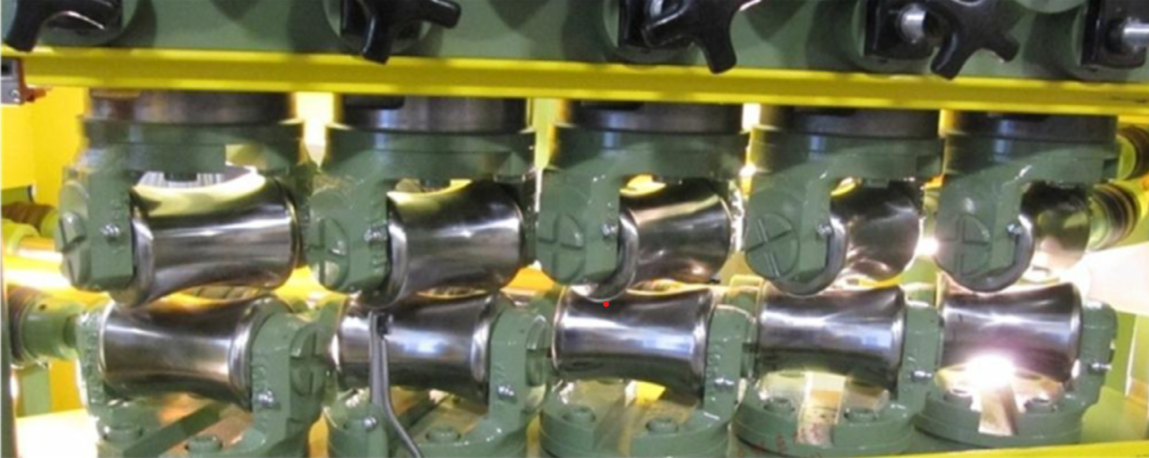
\includegraphics[width=\textwidth, keepaspectratio]{Straightening6.png}
	\caption[Image of a 10 roller straightening machine]{Image of a 10 roller straightening machine~\cite{zhang2019modeling}}
	\label{straighteningImage6}
\end{figure}

\section{Theory}
\subsection{Feature Extraction}
%Why Feature Extraction?
Machine learning algorithms suffer from high amounts of data and information redundancy while requiring vast amounts of storage. Feature extraction, the process of computing numerical values from raw signals, is one method that can be used to combat these issues. By extracting signal features and deciding which are irrelevant one can reduce the amount of data that needs to be stored and processed while still retaining the essence of the signals.

%Feature extraction used in condition monitoring/degradation
Feature extraction techniques are commonly used to estimate degradation trends in machines~\cite{caesarendra2017review,adams2017comparison,hong2014condition}.
%Types of features
Features can include time domain, frequency domain, time-frequency domain (temporal) and model based methods~\cite{teti2010advanced}. Some of the most widely used and effective time domain indicators are mainly based on \gls{RMS}, crest factor, and kurtosis~\cite{soualhi2021novel}. Time-frequency values are three dimensional features which include wavelet analysis, spectrograms, scalograms, Wigner-Ville distribution, and kurtograms~\cite{soualhi2021novel}.~\cite{d2019physical} proposes a feature set built on experimental data from sensors plus results from building a simplified kinematic and dynamic model.

Machine \gls{CM} can utilize various form of sensors and signals including: vibration monitoring, acoustic emission monitoring, a fusion of vibration and acoustic, electric motor current monitoring, oil analysis, thermography~\cite{ahmed2020condition}. There is no one size fits all when it comes to condition monitoring. For a slewing bearing, which is a large low-speed heavy-load bearing, vibration signals are insufficient~\cite{wang2016multiple} and thus fusion models based on torque, temperature and vibration are needed.

\subsection{Signal Features} 	
A non exhaustive list of features, in particular the ones used in this project, are as follows~\cite{diagnosticFeatureDesigner}:

%Mean
The mean, $ \bar{x} $, is the average value of the signal,
\begin{equation}
\bar{x} = \frac{\sum^N_{i=1} x_i}{N},
\end{equation}
where $ x_i $ is the $ i $:th element of the signal and $ N $ is the number of samples in the signal.

%Standard Deviation
The standard deviation, $\sigma$, is the square root of variance, and measures the dispersion of a data set relative to its mean,
\begin{equation}
	\sigma = \sqrt{\frac{\sum^N_{i=1}(x_i-\bar{x})^2}{(N-1)}}.
\end{equation}

%RMS
\gls{RMS} is the square root of the mean squared,
\begin{equation}
x_{RMS} = \sqrt{\frac{1}{N} \sum^N_{i=1}x^2_i}.
\end{equation}
Excessive variation in the \gls{RMS} level usually means a change in health status and possible failure.
 
%Shape Factor
Shape factor is the root mean square divided by the mean of the absolute value,
\begin{equation}
x_{SF} = \frac{ x_{RMS} }  {\frac{1}{N}\sum^N_{i=1}|x_i|}.
\end{equation}
It is dependent on the signal shape and independent of the scale of the signal.

%Kurtosis
Kurtosis is derived from the statistical moment of the fourth order and is defined as the ratio between the mean value of the signal raised to the power of 4 and the square of its variance, \begin{equation}
x_{kurt} = \frac{\sum^N_{i=1}(x_i-\bar{x})^4}{(N-1)\sigma^4}.
\end{equation}
It is  used to analyze the flattening of a distribution and observe the shape of the signal. It is a statistical measure of the tailedness of a distribution and indicates the total degree of outliers present. An increase in the number of outliers, and thus an increase in the Kurtosis, can be a indication of an impending fault. For normal bearing operation, kurtosis is close to 3 and increases rapidly with failure.

%Skewness
Skewness is a measure of asymmetry in the probability density function,
\begin{equation}
x_{skew} = \frac{\sum^2_{i=1}(x_i-m)^3}{(N-1)\sigma^3}.
\end{equation}
Faults can sometimes be revealed through asymmetric distribution.

%Peak Value
The maximum value of a signal,
\begin{equation}
x_p = \textrm{max}(x_i),
\end{equation}
where $x_p$ is the peak value of a signal.

%Impulse Factor
The maximum absolute value divided by the mean of absolute value,
\begin{equation}
x_{IF} = \frac{x_p}{\frac{1}{N}\sum^N_{i=1}|x_i|},
\end{equation}
in other words a comparison of the height of the peak to the average value.

%Crest Factor
Crest Factor is found by dividing the maximum absolute value of a signal by the \gls{RMS} value,
\begin{equation}
x_{crest} = \frac{x_p}{\sqrt{\frac{1}{N}\sum^N_{i=1}x^2_i}}.
\end{equation}
Faults can often be detected as a peakiness of signals before they become evident in the energy (\gls{RMS}). Other indicators have been developed based on the crest factor, such as the K-factor, by multiplying the peak value by the rms value or the peak-to-peak value, measuring the difference between the amplitudes of the upper and lower peaks~\cite{soualhi2021novel}.

%Clearance Factor
Clearance factor is the defined as the peak value divided by the squared mean value of the square roots of the absolute values,
\begin{equation}
x_{clear} = \frac{x_p}{(\frac{1}{N}\sum^N_{i=1}\sqrt{|x_i|})^2}.
\end{equation}
For a healthy bearings this feature is maximum and decreases as faults develop.

The next features come from the frequency domain and one must first calculate the \gls{FFT} before computing the features themselves.
%SNR
\gls{SNR} is the ratio of signal power to noise power in decibels,
\begin{equation}
	SNR = 10 \textrm{log}_{10} \frac{P_{signal}}{P_{noise}},
\end{equation}
where $P_{signal}$ is the average power of the signal and $P_{noise}$ is the average power of the noise.
%   R = SNR(X) computes the signal to noise ratio (SNR), in dBc, of the
%   real sinusoidal input signal X. The computation is performed over a
%   periodogram of the same length as the input using a Kaiser window and
%   excludes the power of first six harmonics (including the fundamental).

%SINAD
\gls{SINAD} is the ratio of total signal power to total noise-plus-distortion power,
\begin{equation}
	SNR = 10 \textrm{log}_{10} \frac{P_{signal} + P_{noise} + P_{distortion}}{P_{noise} + P_{distortion}}, 
\end{equation}
where $P_{signal}$ is the average power of the signal, $P_{noise}$ is the average power of the noise and $P_{distortion}$ the average power of the distortion.

\gls{THD} is calculated as the ratio of total harmonic power to fundamental power,
\begin{equation}
	THD = \frac{P_{h}}{P_{f}} = \frac{\sqrt{P^2_{h2} + \hdots + P^2_{hN}}}{P_1},
\end{equation}
where $P_{f}$ is the power of the fundamental frequency and $P_{h}$ is the power of the the remaining harmonics. $P_N$ is the $N$:th harmonic of the \gls{FFT} and MATLAB takes the first five harmonics using a modified periodogram of the same length as the input signal. The modified periodogram uses a Kaiser window.

\subsection{Spectral Features}
In order to compute spectral features one must first compute the power spectral density which indicates the distribution of power per unit frequency. MATLAB does this via periodogram method. It then uses the command, 'findpeaks', to locate the maximum values of the power spectrum. A local peak is classified as a sample which is either larger than the two neighboring samples or is equal to infinity. Two features come directly from the peak data 1)
%Peak Frequency
Peak Frequency is the value of the frequency which has the highest peak and 2)
%Peak Amplitude
Peak Amplitude is the height of this same peak on the power spectrum.
%Band Power
The Band Power is the area beneath the power spectral density graph, within a selected frequency range. MATLAB uses the command, 'trapz', to compute the approximate integral of the signal via the trapezoidal method with unit spacing.

\subsection{$R^{2}$ correlation}
The coefficient of determination, or $R^{2}$ correlation, is a measure of how well a model predicts the actual output values. It is calculated as the one minus the \gls{SSR} divided by \gls{TSS},

\begin{comment}
%R^{2} = 1 - \frac{\textrm{SSR}}{\textrm{TSS}} = 1 - \frac{\sum^N_{i=1}(x_i - \hat{x_i})^2}{\sum^N_{i=1}(x_i - \bar{x_i})^2},
\end{comment}
\begin{equation}
R^{2} = 1 - \frac{\textrm{RSS}}{\textrm{TSS}} = 1-\frac{\sum^N_{i=1}(y_i - \hat{y_i})^2}{\sum^N_{i=1}(y_i - \bar{y})^2},
\end{equation}
where $y_i$ is the $i$:th output, $\hat{y_i}$ is the predicted value of the model and $\bar{y}$ is the mean of $y$~\cite{james2013introduction}. An $R^{2}$ value of 1 means that the two signals are perfectly identical expect for a multiplicative constant and a value of zero means there is no linear relationship. A value between 0 and 1 indicates some degree of linear relationship exists with the degree of linearity increasing with the value.
        
\subsection{Feature Selection}
Once features have been calculated the challenge is to isolate the most useful and relevant features. Often data sets contain irrelevant, highly correlated or noisy features that can be removed without a significant loss of information. Ideally non-informative and redundant features are removed to reduce complexity, making models easier to interpret. To this point,~\cite{tolocsi2011classification} argues that several widely used classification algorithms can generate misleading feature rankings when the training datasets contain large groups of correlated features. Considering all the research, there is no consensus on which feature/combination of features are best suited for the identification of and distinguishing between faults. 

%Techniques for selecting features
% Best subset selection (forward/backward step-wise selection)
A common method for selecting the most suitable features is forward or backward step wise selection~\cite{james2013introduction}. Forward selection begins with a null model and creates simple linear regressions for each feature on it's own and the model with the lowest RSS is selected. Using that model as a starting point for the next stage another variable is added to create a number of 2 variable models with the lowest RSS being selected to more forward. This process is continued until some stopping rule is satisfied.

% PCA
\gls{PCA} appears to be another popular technique used in feature selection. In one study, PCA is used to fuse multiple features in order to obtain a bearings state~\cite{lu2016degradation}. Another study uses a PCA-based approach to selecting the most representative features for the classification of defective components and defect severity in three types of rolling bearings~\cite{malhi2004pca}. 

Among other techniques~\cite{buckley2023feature} uses recursive feature elimination and feature correlation clustering, the latter involves using thresholds and removing highly correlation features. Usually some kind of goodness of fit metric is used to compare feature models, Zang proposes a combination of correlation, monotonicity and robustness for feature selection~\cite{zhang2016degradation}.

%Acoustic emission signals were extracted both by discrete wavelet decomposition and autoregressive modeling. The three feature selection methods include the sequential forward floating selection, and two ant colony optimization-based feature selection methods~\cite{liao2010feature}.

\subsection{Linear Regression Models}
Once a subset of features has been selected linear models can be created between two features,
\begin{equation} \label{eq:linearModel}
	\mathbf{Y} = \boldsymbol{\uptheta} \mathbf{X},
\end{equation}
where $\mathbf{X}$ is the input vector (or the feature 1), $\mathbf{Y}$ is the output vector of the model (or feature 2) and $\boldsymbol{\uptheta}$ are the model values. By plotting one signal feature against another signal feature, linear relationships in the data can be revealed. Not only linear relations but quite possibly non-linear relationships too. The parameters, $\boldsymbol{\uptheta}$, of the linear model are estimated using linear least squares, 
\begin{equation} \label{eq:regression}
	\hat{\boldsymbol{\uptheta}} = (\mathbf{X}^{\textrm{T}} \mathbf{X})^{-1} \mathbf{X}^{\textrm{T}} \mathbf{Y},
\end{equation}
where $ \hat{\boldsymbol{\uptheta}} = \begin{bmatrix} \hat{\theta_{1}} \\ \vdots \\ \hat{\theta_{n}} \end{bmatrix} $, $ \mathbf{X} = \begin{bmatrix} x_{1}(1) & \hdots & x_{k}(1) \\ \vdots & \ddots & \vdots \\ x_{1}(n) & \hdots & x_{k}(n)  \end{bmatrix}$ and 
$ \mathbf{Y} = \begin{bmatrix} y(1) \\ \vdots \\ y(2)\end{bmatrix}$ ~\cite{james2013introduction}.\\
Equation \ref{eq:regression} is used for multivariate models as well as two variable models. Once a model has been calculated a normalized goodness of fit function~\cite{gonzalez2023time}, \gls{NRMSE}, can be used to assess the accuracy of the model,
% Fit equation from compare function
\begin{equation}
	NRMSE = 100 \times \frac{ 1 - \lVert\mathbf{Y} - \mathbf{\hat{Y}}\rVert } { \lVert \mathbf{Y} - \mathbf{\bar{Y}} \rVert },
\end{equation}
where $\mathbf{Y}$ is an $(N \times 1)$ vector containing the the original feature signal selected as the model output, $\mathbf{\hat{Y}}$ is an $(N \times 1)$ vector containing the model’s output, $\mathbf{\bar{Y}}$ is an $(N \times 1)$ vector containing the mean value of $\mathbf{Y}$ and ||.|| denotes the Euclidean norm.

\subsection{Classification and Clustering}
In a perfect world, data would be available for every kind of failure mode possible on a machine. If this were true, supervised learning could be used to train an algorithm to recognize all kinds of degradation conditions and faults. One could build a model that predicts or estimates degradation metrics quite easily based on one or more inputs. This is often not the case and a more likely situation is where a number inputs or parameters exists but no quantitative outputs. However, one can still learn about the relationships between signals and the structure from such data using unsupervised learning. The aim here is to identify patterns in the input-output signals from unlabeled data. Thus, it is useful for modeling complex data for which prior knowledge is hard to get~\cite{martin2017unsupervised}.

Unsupervised learning is more of an inference task rather than prediction. Techniques such as auto-encoders, K-means clustering and sparse coding are used to find clusters and patters. Once feature models have been created, one can often find different clustering of data when a machine is in a degraded condition compared to a healthy state.

%Often we are forced to do unsupervised learning since we don't have failure data
Many studies are performed in the lab on specially constructed test rigs which are built to run until destruction~\cite{soualhi2021novel, wang2016multiple, d2019physical, malhi2004pca}. This is not possible on an operational asset since a company cannot afford to run the machine until it fails. For this reason studies into \gls{CM} of real life machines are often forced to implement unsupervised learning as opposed to supervised.

\begin{comment}
These references haven't been used yet.

A new feature extraction approach using improved symbolic aggregate approximation for machinery intelligent~\cite{zhang2019new}

Automatic feature extraction and selection for condition monitoring and related datasets~\cite{schneider2018automatic}

Comparison of automated feature selection and reduction methods on the condition monitoring issue~\cite{de2018comparison}

Condition monitoring method for the detection of fault graduality in outer race bearing based on vibration-current fusion, statistical features and neural network~\cite{saucedo2021condition}

This paper talks about "top sensitive features" [Feature extraction, condition monitoring, and fault modeling in semiconductor manufacturing systems]~\cite{bleakie2013feature}.

Features selection procedure for prognostics: An approach based on predictability [Features selection procedure for prognostics, an approach based on predictability]~\cite{javed2012features}

Heterogeneous feature models and feature selection applied to bearing fault diagnosis~\cite{rauber2014heterogeneous}

Multifeatures fusion and nonlinear dimension reduction for intelligent bearing condition monitoring~\cite{guo2016multifeatures}

Optimal symbolic entropy: An adaptive feature extraction algorithm for condition monitoring of bearings~\cite{li2023optimal}

"This paper addresses this issue with an application to tool condition monitoring in
milling, where classifiers based on support vector machines and random forest were employed."~\cite{assafo2023stability}
\end{comment}
\clearpage
  
\section{Data Processing}
\subsection{Description of Data}
The data provided by Alleima consists of approximately a one hour period of data each day over a 15 day duration. It is assumed that it was taken from the same period of time each day. The data was captured by an Iba-DAQ data acquisition system with a sampling time 0.02 seconds ~\cite{ibaMDAQ}. The list of channels provided are shown in Table \ref{signalNames}.
\begin{center}
\captionof{table}{Signal Names}\label{signalNames}
\begin{tabular}{ |c|c|l| }
 \hline
Signal Index & Signal Number & Signal Name \\ 
 \hline
1 & 21:07 & Angle over rolls [deg] \\
 \hline
2 & 21:10 & Position over rolls [mm] \\
 \hline
3 & 21:12 & Actual moment over rolls [Nm] \\
 \hline
4 & 21:17 & Angle under rolls [deg] \\
 \hline
5 & 21:20 & Actual moment under rolls [Nm] \\
 \hline
6 & 21:28 & Vibration measurements [mm/s] \\ 
 \hline              
7 & 21:31 & Width position [mm] \\
 \hline
8 & 21:32 & Height position [mm] \\
 \hline
9 & 21:33 & Error position for height [mm] \\
 \hline
10 & 21:34 & Error position for the width [mm] \\
 \hline
11 & 21:35 & Set point force [kN] \\
 \hline
12 & 21:36 & Actual force [kN] \\
 \hline
\end{tabular}
\end{center}

\subsection{Pre-processing}
State detection for this application is performed using the Signal 5, 21:20 Actual moment under rolls. This was suggested by the team at Alleima, who have expert knowledge with the system, as the most appropriate signal to use. When the machine is not actively processing a tube this value is much less than when it is processing a tube. When no tube is in the system there is none or minimal torque on this sensor and when processing it experiences a much larger moment. The data is separated into cycles using this signal to isolate the periods where the machine is in the act of processing a part. A threshold of 500 samples, 10 seconds, was used to filter out short pulses which aren't believed to be full cycles.

\Cref{fig:StateDetection} shows the windows that were identified from each file where the 21.20 signal was above the threshold. Two files, B\_30\_03 and B\_04\_04, contained no identified pulses. In total 240 pulses were identified where the 21.20 signal crosses the threshold. Any pulse under 500 samples was removed from the data for the next stage leaving 224 pulses to extract features from.

\begin{figure}[H]
    \centering
    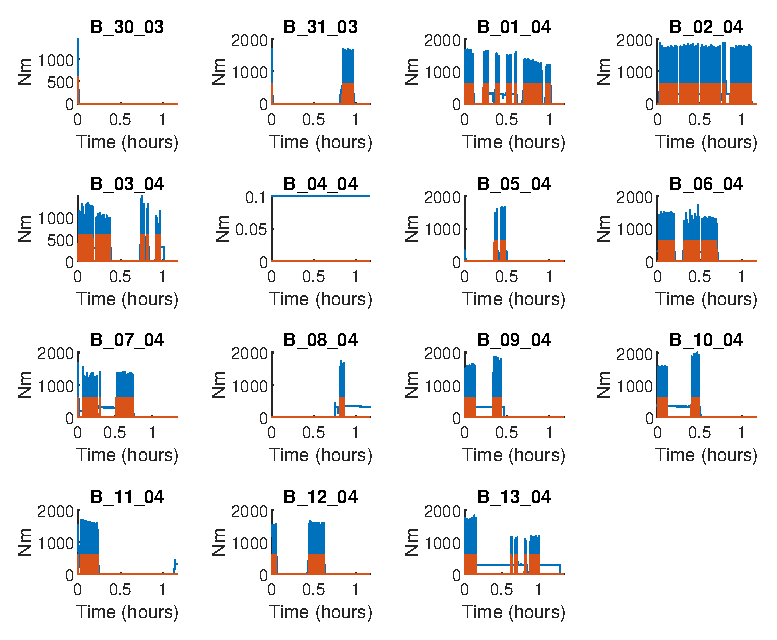
\includegraphics[width=\textwidth, height=\textheight, keepaspectratio]{figures/StateDetectionFig.eps}
    \caption{Signal 5 21:20 Actual moment under rolls and State Detection}
    \label{fig:StateDetection}
\end{figure}

\Cref{fig:StateDetectionFig_B_02_04} shows one of the plots from \cref{fig:StateDetection}, B\_02\_04, in greater detail. This particular file is the one with the highest number of pulses.

\begin{figure}[H]
    \centering
    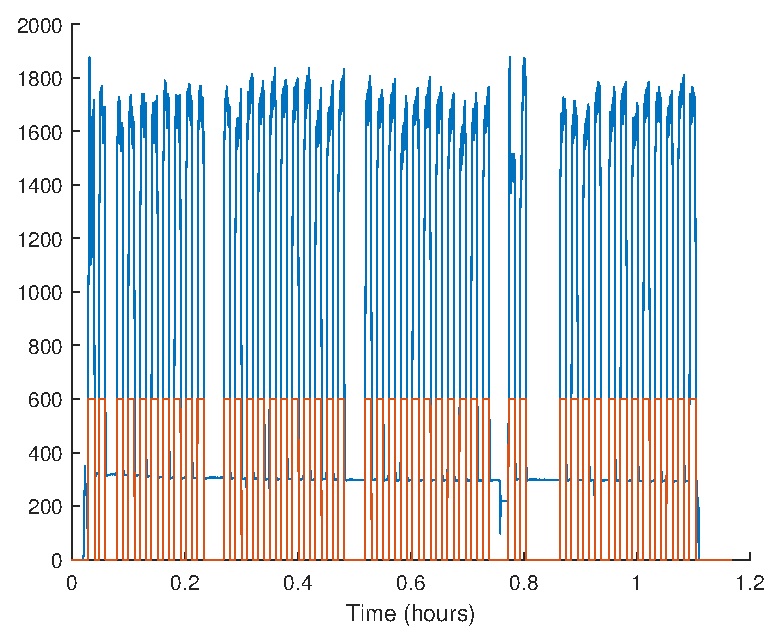
\includegraphics[scale=0.75]{figures/StateDetectionFig_B_02_04.eps}
    \caption{State detection for signal 21:20 performed on file B\_02\_04}
    \label{fig:StateDetectionFig_B_02_04}
\end{figure}

\Cref{fig:IdentifiedPulses} shows pulses or cycles for Signal 5, 21:20, in each of the fifteen files. As mentioned earlier B\_30\_03 and B\_04\_04 show no pulses as all. All the pulses are around 40 seconds in duration with similar shapes but varying profiles.
 
\begin{figure}[H]
    \centering
    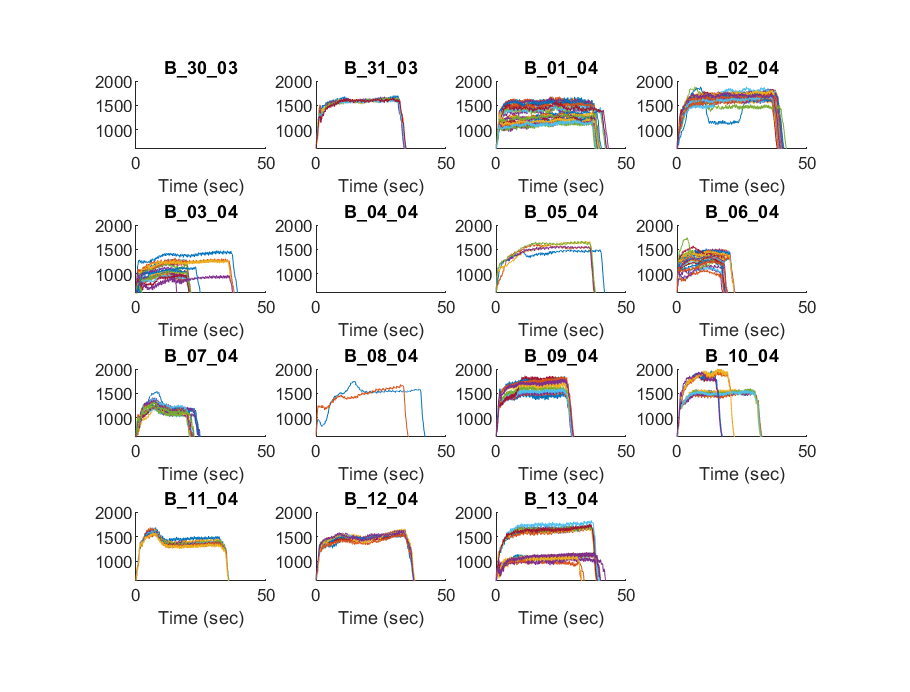
\includegraphics[width=\textwidth, height=\textheight, keepaspectratio]{figures/IdentifiedPulsesFig.eps}
    \caption{Identified pulses in each files for file}
    \label{fig:IdentifiedPulses}
\end{figure}

\Cref{fig:SignalPulses} shows the signals for all 224 pulses with each sensor channel plotted in a different tile. 
\begin{figure}[H]
	\makebox[\textwidth][c]{\includegraphics[width=1.15\textwidth, height=\textheight, keepaspectratio]{figures/SignalPulses.eps}}
    \caption{Signal pulses for 224 cycles on each of the 12 channels}
    \label{fig:SignalPulses}
\end{figure}

Using the identified pulses, one can look at all the other signals during the same periods. Signal 1: 21.07 Angle over rolls and 2: 21.10 Position over rolls are fairly constant though contain some small deviations. Signal 7, 21:31 Width position and 8, 21:32 Height position are also fairly constant but contain some information when the scale is increased. Signal 21.35, Force Set Point is a 100\% constant signal and contains nothing but a single value. Considering the label, it can be assumed that this is a set point that is controlled by the operator or control system and not as sensor on the machine providing feedback. Apart from using this signal for further separating the data into different categories it's likely not that useful for condition monitoring.

\Cref{fig:SignalPulse5} shows the state detection Signal 5, Moment under rolls, in more detail. Visually one can see these are a type of pulse single with a small amplitude frequency component. Signal 3: Moment over rolls looks like a very similar type of signal. Signals 6, 9, 10 and 11 contain some interesting information that can be used for characterize the machine state.

\begin{figure}[H]
    \centering
    \includegraphics[scale = 0.75, keepaspectratio]{figures/SignalPulse5.eps}
    \caption{Signal 5 Pulses 21:20 Actual moment under rolls}
    \label{fig:SignalPulse5}
\end{figure}

\begin{comment}
Additional data sets were created by adding some addition preprocessing steps. One set where the signal mean was subtracted from all the channels and another where zero padding was used to make all the signal lengths are the same. 
%The reason for this ......
\end{comment}

\section{Results}
\subsection{Signal Correlations}
A comparison of the raw signals was performed using $R_2$ values. This was not performed for all files due to the long time taken to run the script, just the ones with the most pulses. Table \ref{correlationTable} shows the $R_2$ values for each pair of signals for file 4, the one with the most pulses, with the lower triangle being a replica of the upper triangle. \Cref{fig:RawSignalCorrelationsFile1} plots all of the signals against each other for file 4 with the $R_2$ values in the range of 0.2 to 0.9 printed on the plots. The colors used in the figure are used to represent the time scale with the start of the time scale being blue and trending towards red.

Starting with some basic observations from \cref{fig:RawSignalCorrelationsFile1}, there are a few combinations that are extremely linear. Two pairs that are highly correlated are:
\begin{enumerate}
\item Signal 7, 21:31 Width position and Signal 10, 21:34 Error position for width.
\item Signal 8, 21:32 Height position and Signal 9, 21:33 Error position for height.
\end{enumerate}
These data pairs appear to form a V shape with two straight lines meeting at a point. Intuitively this makes sense because the error signals themselves are fairly constant with very small variation. As the height/width position increases or decreases further away from the set point the larger or smaller the error gets. Therefore these two pairs should always be highly correlated.  

Signal 3, 21:12 Actual moment over rolls and Signal 5, 21:20 Actual moment under rolls are also highly linear. This would indicate that the torque on both dimensions of the pipe are varying together.

One signal that is of interest is Signal 6, 21:28 Vibration Measurements, and two combinations it forms with Signal 3, Actual moment over rolls and Signal 5, Actual moment under rolls. Both these combinations have the same correlation value and when looking at \cref{fig:RawSignalCorrelationsFile1} there appears to be a clear non-linear relationship.

\Cref{fig:RawSignalCorrelationsFile1_Caption} shows more clearly what could be an exponential or cubic relationship between the vibrations and the torque values on the upper and lower rollers. The four plots are of the four files with the most pulses and all appear to have similarities in shape. This could be explained by the fact that the larger vibration of the rollers the more torque is experienced or applied by the actuators to keep the rollers in place. \Cref{fig:File3_Signal3vSignal6} shows what could be a time dependent relationship since the colors trend from red to blue on the right side of the plot but this is not really evident in the other plants. 

While \cref{fig:RawSignalCorrelationsFile1_Caption} plots the Signal 3, Moment over rolls, against Signal 6 it should be noted that the plots for Signal 5, Moment under rolls look very similar but are not included in the report. It is also worth to remember that File 1 and 6 contain no identified pulses so the $R_2$ tables for those two files, while not included in the report, look quite different to the others and should be ignored.

\begin{center}
\captionof{table}{$R_2$ values for each signal vs. each other signal}
\begin{scriptsize}
\begin{tiny}\begin{tabular}{|l|c|c|c|c|c|c|c|c|c|c|c|c|}
\hline
&\textbf{07}&\textbf{10}&\textbf{12}&\textbf{17}&\textbf{20}&\textbf{28}&\textbf{31}&\textbf{32}&\textbf{33}&\textbf{34}&\textbf{35}&\textbf{36}\\\hline
\textbf{07}&1.00&0.07&0.00&0.01&0.00&0.02&0.04&0.45&0.46&0.03&-Inf&0.00\\\hline
\textbf{10}&0.07&1.00&0.02&0.00&0.02&0.00&0.23&0.15&0.14&0.19&-Inf&0.00\\\hline
\textbf{12}&0.00&0.02&1.00&0.02&1.00&0.47&0.02&0.00&0.00&0.01&-Inf&0.01\\\hline
\textbf{17}&0.01&0.00&0.02&1.00&0.02&0.22&0.00&0.00&0.00&0.00&-Inf&0.01\\\hline
\textbf{20}&0.00&0.02&1.00&0.02&1.00&0.46&0.01&0.00&0.00&0.01&-Inf&0.01\\\hline
\textbf{28}&0.02&0.00&0.47&0.22&0.46&1.00&0.02&0.01&0.01&0.03&-Inf&0.00\\\hline
\textbf{31}&0.04&0.23&0.02&0.00&0.01&0.02&1.00&0.17&0.15&0.99&-Inf&0.04\\\hline
\textbf{32}&0.45&0.15&0.00&0.00&0.00&0.01&0.17&1.00&0.99&0.14&-Inf&0.00\\\hline
\textbf{33}&0.46&0.14&0.00&0.00&0.00&0.01&0.15&0.99&1.00&0.13&-Inf&0.00\\\hline
\textbf{34}&0.03&0.19&0.01&0.00&0.01&0.03&0.99&0.14&0.13&1.00&-Inf&0.04\\\hline
\textbf{35}&-0.00&-0.00&-0.00&0.00&-0.00&0.00&-0.00&-0.00&0.00&0.00&-Inf&-0.00\\\hline
\textbf{36}&0.00&0.00&0.01&0.01&0.01&0.00&0.04&0.00&0.00&0.04&-Inf&1.00\\\hline
\end{tabular}
\end{tiny} 
\end{scriptsize}
\label{correlationTable}
\end{center}

\begin{figure}[H]
    \centering
    \includegraphics[width=\textwidth, height=\textheight, keepaspectratio]{figures/RawSignalCorrelationsFile4.eps}
    \caption{Plot of each signal vs every other signal with $R_2$ values between 0.2 and 0.9 for File 4}
    \label{fig:RawSignalCorrelationsFile1}
\end{figure}


\begin{figure}[H]
	\captionsetup[subfigure]{}
    \centering
		\begin{subfigure}{.45\textwidth}
		  	\centering
    			\includegraphics[width=\linewidth]{figures/File3_Signal3vSignal6.eps}
		  	\caption{File 3}
		  	\label{fig:File3_Signal3vSignal6}
		\end{subfigure}
		\hspace{\fill}
		\begin{subfigure}{.45\textwidth}
		  	\centering
 		   	\includegraphics[width=\linewidth]{figures/File4_Signal3vSignal6.eps}
		  	\caption{File 4}
		  	\label{fig:File4_Signal3vSignal6}
		\end{subfigure}  
	\bigskip    
    \centering
		\begin{subfigure}{.45\textwidth}
		  	\centering
    			\includegraphics[width=\linewidth]{figures/File8_Signal3vSignal6.eps}
		  	\caption{File 8}
		  	\label{fig:File8_Signal3vSignal6}
		\end{subfigure}
		\hspace{\fill}
		\begin{subfigure}{.45\textwidth}
		  	\centering
 		   	\includegraphics[width=\linewidth]{figures/File13_Signal3vSignal6.eps}
		  	\caption{File 13}
		  	\label{fig:File13_Signal3vSignal6}
		\end{subfigure}
    \caption{Vibration vs Moment where color equates to time over approximately 1 hour}
    \label{fig:RawSignalCorrelationsFile1_Caption}    
\end{figure}

\subsection{Feature Selection}
Once the data has been pre-processed the feature values are calculated for each identified production cycle. For every channel, the $R_2$ value for every pair of signal features is computed and the pairs of data points for each cycle are plotted against each other in a scatter plot. This is used as a first stage for filtering out irrelevant data. A small, or zero, $R_2$ value indicates that there is a very weak or no linear relationship between that pair of features. On the other hand an $R_2$ value of close to 1 indicates that the two features are perfectly or close to perfectly linear.

Two threshold values are used to select a range of $R_2$ correlated features with this method. An upper and and a lower $R_2$ threshold value are specified which reveals feature pairs which are somewhat linear or varying in nature. These are the combinations that are of interest to look for condition indicators.

A semi automated method is be used to narrow down on feature pairs of interest. An algorithm cycles through the table of $R_2$ values and the features correlated to a number of others can be isolated. Within that combination one can then remove those signals from the group which are highly correlated with each other. Not only can one compare pairs of features within the same signal but one can also look for relationships between the same feature over multiple channels. A manual approach was then used to select a few relationships of interest to include in the report.

MATLAB's Diagnostic Feature Designer was used calculate the features from the signal pulse data with Table \ref{signalNames} showing the features that were extracted. Throughout the remainder of the report some figures are labeled with a feature number instead of the full text due to readability and space constraints. Use Table \ref{signalNames} to refer to which feature the indexes represents.

\begin{center}
\captionof{table}{Feature Names}\label{featureNames}
\begin{tabular}{ |c|l|c|l| }
 \hline
 1 & Clearance Factor & 9 & \gls{SINAD}\\
 \hline
 2 & Crest Factor & 10 & Shape Factor\\
 \hline
 3 & Impulse Factor & 11 & Skewness\\
 \hline
 4 & Kurtosis & 12 & Standard Deviation\\
 \hline
 5 & Mean & 13 & \gls{THD}\\
 \hline
 6 & Peak Value &  14 & Band Power \\
 \hline
 7 & \gls{RMS} & 15 & Peak Amplitude 1\\ 
 \hline              
 8 & \gls{SNR} & 16 & Peak Frequency 1 \\
 \hline        
\end{tabular}
\end{center}

\subsection{Feature vs Feature Models}
\Cref{fig:FeatureVsFeatureCombinedSignal3} shows an example of plotting all features against one another. This was repeated for all signals, one is shown in the main section of this report, the rest can be found in Appendix \ref{appendix:Plots}. Each number on the diagonal represents a feature from Table \ref{signalNames}, starting with the signal features followed by the spectral features. Only the $R_2$ values between 0.3 and 0.8 are printed on the relevant plots. The colors used in these plots are used to represent a pseudo time scale. Since the data is only from 1 hour per day the color spectrum is non linear however it may be useful in revealing any trends over time.

Once a subset of features are chosen, equation \ref{eq:linearModel} is used to create a model. If two features are selected, for example kurtosis and mean, then the model is given by
\begin{equation}
\mathbf{X}_{\textrm{kurtosis}} = \boldsymbol{\uptheta}'\mathbf{X}_{\textrm{mean}}
\end{equation}
where $\mathbf{X}_{\textrm{kurtosis}}$ is an $(N\times1)$ array, $\boldsymbol{\uptheta}$ is a $(2\times1)$ array and $\mathbf{X} = \begin{bmatrix} 1 & \mathbf{X}_{\textrm{mean}}(1) \\ \vdots & \vdots \\ 1 & \mathbf{X}_{\textrm{mean}}(N) \end{bmatrix}$, which is an $(N\times2)$ matrix. 

%\subsubsection*{Signal 3 21:12 Actual moment over rolls}
It can be noted in \cref{fig:FeatureVsFeatureCombinedSignal3} that Features 1, 2 and 3 all have very straight lines so here we can say that these features (Clearance, Crest and Impulse Factor), are linearly correlated and thus need only include one of these in any model. This is the same situation for Features 5, 6 and 7 (Mean, Peak Value and RMS).
Looking at Feature 14, Band Power, it can be seen that the $R_2$ value is within the specified range when compared with Features 10 and 12. \Cref{fig:Models_Signal3Feature14} shows these three features plotted against one another for all cycles. As expected they are somewhat similar in pattern but not exactly the same. Linear regression models were created, \cref{fig:Models_Signal3Feature14_Linear1,fig:Models_Signal3Feature14_Linear2} with the \gls{NRMSE} value shown in the plots. \Cref{fig:Models_Signal3Feature14_Multivariate1} shows a three dimensional model for all three of those Features which looks extremely linear apart from a few outlines. The \gls{NRMSE} value is increased from the individual plots which means it's a pretty good fit. It's also worth to note, while the figures are not included in the report, Signal 5 21:20 Actual moment over rolls has the same characteristics of Signal 3, Actual moment under rolls which means one can not make an assumption that the variance is constant along the signal.

\begin{figure}[H]
    \centering
    \includegraphics[width=\textwidth, height=\textheight, keepaspectratio]{figures/FeatureVsFeatureCombinedSignal3.eps}
    \caption{Feature vs Feature for Signal 3, 21:12 Actual moment over rolls}
    \label{fig:FeatureVsFeatureCombinedSignal3}
\end{figure}

\begin{figure}[H]
	\captionsetup[subfigure]{}
    \centering
		\begin{subfigure}{.45\textwidth}
		  \centering
    			\includegraphics[width=.95\linewidth]{figures/Models_Signal3Feature14.eps}
		  	\caption{Feature values over time: Shape Factor (blue), Standard Deviation (blue) and Band Power (red).}
		  	\label{fig:Models_Signal3Feature14}
		\end{subfigure}\hspace{\fill}% 
		\begin{subfigure}{.45\textwidth}
		  \centering
 		   	\includegraphics[width=.95\linewidth]{figures/Models_Signal3Feature14_Linear1.eps}
		  	\caption{Band power vs Shape factor with data points in color ordered in time and linear model in red with \gls{NRMSE} = 26.2.}
		  	\label{fig:Models_Signal3Feature14_Linear1}
		\end{subfigure}
		\bigskip
		\begin{subfigure}{.45\textwidth}
		  \centering
    			\includegraphics[width=.95\linewidth]{figures/Models_Signal3Feature14_Linear2.eps}
		  	\caption{Band power vs Standard Deviation with data points in color ordered in time and linear model in red with \gls{NRMSE} = 48.1.}
		  	\label{fig:Models_Signal3Feature14_Linear2}
		\end{subfigure}\hspace{\fill}%
		\begin{subfigure}{.45\textwidth}
		  \centering
 		   	\includegraphics[width=.95\linewidth]{figures/Models_Signal3Feature14_Multivariate1.eps}
		  	\caption{Multivariate Model of Shape Factor, Standard Deviation and Band Power with \gls{NRMSE} = 61.5.}
		  	\label{fig:Models_Signal3Feature14_Multivariate1}
		\end{subfigure}
    \caption{Signal 3, 21:12 Actual moment over rolls}
    \label{fig:Models_Signal3Feature14_Caption}
\end{figure}



%\subsubsection*{Signal 5 Actual moment under rolls}



%\subsubsection*{Signal 6, Vibration Measurements}
The vibration features in \cref{fig:Models_Signal6Feature2_Caption} shows an interesting relationship. Five of the features are have correlation values within the specified range but one combination in particular has a different relationship to the others. The Crest Factor vs Band Power exhibits a relationship with an increasing variance. 
\begin{figure}[H]
    \centering
		\begin{subfigure}[t]{.45\textwidth}
		  	\centering
    			\includegraphics[width=.95\linewidth]{figures/Models_Signal6Feature2.eps}
		  	\caption{Feature values over time: Crest Factor (blue), Mean (red), Shape Factor (blue dashed), Skewness (blue dotted) and Band power (blue dash-dotted).}
		  	\label{fig:Models_Signal6Feature1}
		\end{subfigure}\hspace{\fill}% maximize horizontal separation
		\begin{subfigure}[t]{.45\textwidth}
		  	\centering
 		   	\includegraphics[width=.95\linewidth]{figures/Models_Signal6Feature2_Linear4.eps}
		  	\caption{Crest factor vs Band power with data points in color ordered in time and linear model in red with \gls{NRMSE} = 33.7.}
		  	\label{fig:Models_Signal6Feature2_Linear4}
		\end{subfigure}
    \caption{Signal 6, 21:28 Vibration measurements}
    \label{fig:Models_Signal6Feature2_Caption}
\end{figure}



%\subsubsection*{Signal 9, Height Error}
Looking at the error for the height position, there is an an interesting pattern in the data for Feature 7, \gls{RMS}. \Cref{fig:Models_Signal9Feature7} shows a number of the correlated features drawn on the same plot however the combination of \gls{RMS} and Standard Deviation is the one of interest. \Cref{fig:Models_Signal9Feature7_Linear4} shows these two features plotted against each other and there is a straight line clearly apparent however some other little clusters appear adjacent to this line. The straight line could represent when the machine is working in a good operating window and the clusters when it deviates from this.
\begin{figure}[H]
    \centering
		\begin{subfigure}[t]{.45\textwidth}
		  	\centering
    			\includegraphics[width=.95\linewidth]{figures/Models_Signal9Feature7.eps}
		  	\caption{Feature values over time: Clearance Factor (blue), Peak Value (dotted blue), RMS (red), Shape Factor (dashed red) and Standard Deviation (dotted red).}
		  	\label{fig:Models_Signal9Feature7}
		\end{subfigure}\hspace{\fill}%
		\begin{subfigure}[t]{.45\textwidth}
		  	\centering
 		   	\includegraphics[width=.95\linewidth]{figures/Models_Signal9Feature7_Linear4.eps}
		  	\caption{RMS vs Standard Deviation with data points in color ordered in time and linear model in red with \gls{NRMSE} = 17.9.}
		  	\label{fig:Models_Signal9Feature7_Linear4}
		\end{subfigure}
    \caption{Signal 9, 21:33 Error position for height}
    \label{fig:Models_Signal9Feature7_Caption}
\end{figure}


\Cref{fig:Models_Signal9Feature11_Caption} shows the subset of features for Feature 11, Skewness. Two combinations appear to show exponential relationships, Skewness vs Kurtosis \cref{fig:Models_Signal9Feature11_Linear1} and Skewness vs Shape Factor \cref{fig:Models_Signal9Feature11_Linear3}.
\begin{figure}[H]
	\captionsetup[subfigure]{}
    \centering
		\begin{subfigure}[t]{.45\textwidth}
		  \centering
    			\includegraphics[width=.95\linewidth]{figures/Models_Signal9Feature11.eps}
		  	\caption{Feature values over time: Kurtosis (blue), Mean (red), Shape Factor (dashed red), Skewness (dashed blue) and Peak Frequency (dotted blue).}
		  	\label{fig:Models_Signal9Feature11}
		\end{subfigure}\hspace{\fill} % maximize horizontal separation
		\begin{subfigure}[t]{.45\textwidth}
		  \centering
 		   	\includegraphics[width=.95\linewidth]{figures/Models_Signal9Feature11_Linear1.eps}
		  	\caption{Skewness vs Kurtosis with data points in color ordered in time and linear model in red with \gls{NRMSE} = 41.7.}
		  	\label{fig:Models_Signal9Feature11_Linear1}
		\end{subfigure}
		\bigskip
		\begin{subfigure}[t]{.45\textwidth}
		  \centering
    			\includegraphics[width=.95\linewidth]{figures/Models_Signal9Feature11_Linear2.eps}
		  	\caption{Skewness vs Mean with data points in color ordered in time and linear model in red with \gls{NRMSE} = 17.6.}
		  	\label{fig:Models_Signal9Feature11_Linear2}
		\end{subfigure}\hspace{\fill} % maximize horizontal separation
		\begin{subfigure}[t]{.45\textwidth}
		  \centering
 		   	\includegraphics[width=.95\linewidth]{figures/Models_Signal9Feature11_Linear3.eps}
		  	\caption{Skewness vs Shape Factor with data points in color ordered in time and linear model in red with \gls{NRMSE} = 44.7.}
		  	\label{fig:Models_Signal9Feature11_Linear3}
		\end{subfigure}
    \caption{Signal 9, 21:33 Error position for height}
    \label{fig:Models_Signal9Feature11_Caption}
\end{figure}



%\subsubsection*{Signal 10, Width Error}
\Cref{fig:Models_Signal10Feature11_Caption} plots two features for Signal 10, Width error. \Cref{fig:Models_Signal10Feature11_Linear1} shows a clear non-linear parabolic relationship between the Skewness and the Kurtosis. There could also be a time varying relationship here since the left side of the data set appears to be mostly red and moves to predominantly blue as the skewness increases.
\begin{figure}[H]
    \centering
		\begin{subfigure}[t]{.45\textwidth}
		  \centering
    			\includegraphics[width=.95\linewidth]{figures/Models_Signal10Feature11.eps}
		  	\caption{Feature values over time: Kurtosis (blue) and Skewness (red).}
		  	\label{fig:Models_Signal10Feature7}
		\end{subfigure}
		\hspace*{\fill}%
		\begin{subfigure}[t]{.45\textwidth}
		  \centering
 		   	\includegraphics[width=.95\linewidth]{figures/Models_Signal10Feature11_Linear1.eps}
		  	\caption{Skewness vs Kurtosis with data points in color ordered in time and linear model in red with \gls{NRMSE} = 16.6.}
		  	\label{fig:Models_Signal10Feature11_Linear1}
		\end{subfigure}
    \caption{Signal 10, 21:34 Error position for width}
    \label{fig:Models_Signal10Feature11_Caption}
\end{figure}



%\subsubsection*{Signal 12, Actual Force}
\Cref{fig:Models_Signal12Feature1_Caption} shows two relationships of interest. \Cref{fig:Models_Signal12Feature1_Linear1} appears to be a non-linear exponential relationship where the variance is not constant, but increasing as both values move away from 1. \Cref{fig:Models_Signal12Feature1_Linear2} shows a week linear relationship but appears to have two distinct clusters with one on either side of the plot. The 3D model in \cref{fig:Models_Signal12Feature1_Multivariate1} shows the combination of all three of these variables where there is a dense cluster of data in the lower left of the plot and some clusters of outliers higher up.

\begin{figure}[H]
	\captionsetup[subfigure]{}
    \centering
    
		\begin{subfigure}[t]{.45\textwidth}
		  \centering
    			\includegraphics[width=.95\linewidth]{figures/Models_Signal12Feature1.eps}
		  	\caption{Feature values over time: Clearance Factor (blue), Shape Factor (orange) and Skewness (red).}
		  	\label{fig:Models_Signal12Feature1}
		\end{subfigure}
		\hspace*{\fill}%
		\begin{subfigure}[t]{.45\textwidth}
		  \centering
 		   	\includegraphics[width=.95\linewidth]{figures/Models_Signal12Feature1_Linear1.eps}
		  	\caption{Clearance Factor vs Shape Factor with data points in color ordered in time and linear model in red with \gls{NRMSE} = 59.1.}
		  	\label{fig:Models_Signal12Feature1_Linear1}
		\end{subfigure}
		\bigskip
		\begin{subfigure}[t]{.45\textwidth}
		  \centering
 		   	\includegraphics[width=.95\linewidth]{figures/Models_Signal12Feature1_Linear2.eps}
		  	\caption{Clearance vs Skewness Band power vs Crest factor with data points in color ordered in time and linear model in red with \gls{NRMSE} = 27.5.}
		  	\label{fig:Models_Signal12Feature1_Linear2}
		\end{subfigure}
		\hspace*{\fill}%
		\begin{subfigure}[t]{.45\textwidth}
		  \centering
 		   	\includegraphics[width=.95\linewidth]{figures/Models_Signal12Feature1_Multivariate1.eps}
		  	\caption{Multivariate Model with Shape Factor vs Skewness vs Clearance Factor and a Fit value of 69.9.}
		  	\label{fig:Models_Signal12Feature1_Multivariate1}
		\end{subfigure}
		
    \caption{Signal 12, 21:36 Actual force}
    \label{fig:Models_Signal12Feature1_Caption}
\end{figure}



\subsection{Signal vs Signal Models}
Just as in the last section, where each feature was plotted against every other feature within the same signal, the same thing can be done within a feature. For example we can take the mean of all sensor channels and plot these against each other.

%\subsubsection*{Time Feature 2, Crest Factor}
One feature that was chosen to include in the report is the Crest Factor, \cref{fig:Models_Feature2Signal1_Caption}. \Cref{fig:Models_Feature2Signal9} shows Signal 1 21:07 Angle over rolls vs Signal 6 21:28 Vibrations where the linear model is very accurate close to the Y axis with increasing variance as the Crest Factor of the Angle Over rolls increases.
\begin{comment}
\Cref{fig:SignalVsSignalFeatureFreq3} shows 
\begin{figure}[H]
    \centering
    \includegraphics[width=\textwidth, height=\textheight, keepaspectratio]{figures/SignalVsSignalFeatureFreq3.eps}
    \caption{Signal Vs Signal for Frequency Domain Feature 16 Peak Frequency 1}
    \label{fig:SignalVsSignalFeatureFreq3}
\end{figure}
\end{comment}

\begin{figure}[H]
    \centering
	\begin{subfigure}[t]{.45\textwidth}
		\centering
		\includegraphics[width=.95\linewidth]{figures/Models_Feature2Signal1.eps}
		\caption{Feature values over time: Clearance Factor (blue), Shape Factor (orange) and Skewness (red).}
		\label{fig:Models_Feature2Signal9}
	\end{subfigure}
	\hspace*{\fill}%
	\begin{subfigure}[t]{.45\textwidth}
		\centering
 		\includegraphics[width=.95\linewidth]{figures/Models_Feature2Signal1_Linear1.eps}
		\caption{Angle over rolls vs Vibration with data points in color ordered in time and linear model in red with \gls{NRMSE} = 17.}
		\label{fig:Models_Feature2Signal1_Linear1}
	\end{subfigure}
    \caption{Feature 2 Crest Factor}
    \label{fig:Models_Feature2Signal1_Caption}
\end{figure}



%\subsubsection*{Time Feature 4, Kurtosis}
\Cref{fig:Models_Feature4Signal1_Caption} shows the Kurtosis values for the Height vs the Height Error. It is interesting to note in \cref{fig:Models_Feature4Signal9_Linear1} the there is again increasing variance as the the values increase, but also that there appears to be a cluster of data the forms a very straight line in the lower portion of the graph. This could indicate a certain operating condition and the rest of the data indicates something else. This linear model is valid for errors in Height between 2 to 6mm and height position between 2 to 10mm but outside of these this is not enough data.
\begin{figure}[H]
    \centering
	\begin{subfigure}[t]{.45\textwidth}
		\centering
		\includegraphics[width=.95\linewidth]{figures/Models_Feature4Signal9.eps}
		\caption{Feature values over time: Clearance Factor (blue), Shape Factor (orange) and Skewness (red).}
		\label{fig:Models_Feature4Signal9}
	\end{subfigure}
	\hspace*{\fill}%
	\begin{subfigure}[t]{.45\textwidth}
		\centering
		\includegraphics[width=.95\linewidth]{figures/Models_Feature4Signal9_Linear1.eps}
		\caption{Height Error vs Height Position with data points in color ordered in time and linear model in red with \gls{NRMSE} = 23.8.}
		\label{fig:Models_Feature4Signal9_Linear1}
	\end{subfigure}
    \caption{Feature 4 Kurtosis}
    \label{fig:Models_Feature4Signal1_Caption}
\end{figure}


%\subsubsection*{Frequency Feature 16, Peak Frequency 1}
\Cref{fig:Models_Feature16Signal3_Linear1} shows the peak frequency of the Actual Moment over rolls vs Actual moment under rolls. It can be noted that a majority of the data points follow the a linear model very well. However, a subset of the available data appear to form another linear relationship with a similar gradient but slightly lower intercept.
\begin{figure}[H]
	\centering
	\begin{subfigure}[t]{.45\textwidth}
		\centering
    		\includegraphics[width=.95\linewidth]{figures/Models_Feature16Signal3.eps}
	 	\caption{Feature values over time: Clearance Factor (blue), Shape Factor (orange) and Skewness (red).}
	  	\label{fig:Models_Feature16Signal3}
	\end{subfigure}
	\hspace*{\fill}%
	\begin{subfigure}[t]{.45\textwidth}
	  \centering
 	   	\includegraphics[width=.95\linewidth]{figures/Models_Feature16Signal3_Linear1.eps}
	  	\caption{Actual moment under rolls vs Actual Moment under rolls with data points in color ordered in time and linear model in red with \gls{NRMSE} = 33.6.}
	  	\label{fig:Models_Feature16Signal3_Linear1}
	\end{subfigure}
   	\caption{Feature 16 Peak Frequency 1}
    \label{fig:Models_Feature16Signal3_Caption}
\end{figure}

\clearpage 

\section{Discussion}
% In this chapter the results and the chosen method are discussed, as well as the strengths and weaknesses of the work.
% Discuss results - Comments on what signals are suitable and/or are related
This study aimed to find patterns in the data and  give suggestions as to which signals and signal features are of value for future condition monitoring studies and which are not. Of the data provided, many of the signals were relatively constant showing minimal variance. In particular, Signal 11, 21:35 Set point force is perfectly constant and is not suitable for condition monitoring. The following signals are not overly useful to condition monitoring as they are fairly constant in mean value and contain little variability: 
\begin{itemize}
\item Signal 1, 21:07 Angle over rolls
\item Signal 2, 21:10 Position over rolls
\item Signal 4, 21:17 Angle under rolls
\item Signal 7, 21:31 Width position
\item Signal 8, 21:32 Height position
\item Signal 11, 21:35 Set point force
\end{itemize}

Excluding these signals from future studies already reduces the data by 50\%. The remaining signals are most useful for condition monitoring:
\begin{itemize}
\item Signal 3, 21:12 Actual moment over rolls
\item Signal 5, 21:20 Actual moment under rolls
\item Signal 6, 21:28 Vibration measurements 
\item Signal 9, 21:33 Error position for height
\item Signal 10, 21:34 Error position for the width
\item Signal 12, 21:36 Actual force           
\end{itemize}

%Comment on Method
%Strengths?
The strength in this study lies in using data from an operational machine with varying scales and units. It would be worthwhile to inquire with the company about whether what they have provided is the full set of available signals. Temperature and acoustic emissions are also highly effective types of sensors for condition monitoring so if there was in fact additional data these would be of interest. If none of these sensors exist perhaps it might be a good consideration add one or more of these types of measurements to complement existing infrastructure.

%Weaknesses
The data supplied for the project is from a two week period which probably does not give a good insight into the life cycle of the machine. No maintenance data was provided. Perhaps maintenance is only required on a yearly cycle, thus the data is not full representative of the machine degradation over time. Perhaps a better selection of data would include a snippet of data every 1-2 weeks over a year long period and thus one could get a better view of how the machine degrades over a year.

A system that has been operating for a long period of time will undergo changes due to the natural wear of the system. Ideally, data over the lifespan of a machine would be available. It is not known whether the current data is normal operating data. It could be right at the beginning of the life cycle or could be just at the end of the machines life cycle. 

Throughout the report a color spectrum was used to indicate the time order of pulses in an attempt to reveal degradation conditions. It's worth remembering that this machine processes different sized tubes and thus one could confuse clustering in time with clustering in product sizes. This is where more data broken down in to different product sizes could be better at revealing degradation over time.

%Put in context/comparison with references at the beginning. 
This study utilizes relatively simple methods to in comparison to the types of methods mentioned in earlier sections of the report. An analysis of such data can be expanded exponentially but one can only look at so much. It is also beneficial to, at least begin with, simple things like two variable linear regression and perhaps this is all that is required to identify a indicator of degradation state.

%Enhance scientific research, upgrade the technological capabilities of industrial sectors in all countries, in particular developing countries, including, by 2030, encouraging innovation and substantially increasing the number of research and development workers per 1 million people and public and private research and development spending.
The subject matter, methods and results used in this report are inline with target 9.5 of the 2030 Agenda for sustainable development\cite{united2015department}. Hopefully this work will upgrade technology capabilities in industrial sectors and will assist workers in the field of research and development. 

\subsection{Future Work}
This report has identified patterns in the data and potential clusters based on visual observations. However, no attempts were made to implement any clustering algorithms. This would be the logical next step, to apply machine learning techniques, in trying to identify degradation and failure states.

The straightening machine in this study produces tubes of different diameters. At least one of the signals, Height and/or Width Position, can be used to indicate the diameter. This could be used to classify the data further into different tube widths. A suggestion for future studies is to perform an additional prepossessing step to separate data into periods where the machine is producing tubes with certain diameters. Some of the clustering suggestions or relationships given in this study could just be identifying when the machine is producing a tube of a certain width. Separating data into pipe widths and focusing on only one tube width would remove any chance of this. A method like this would have been challenging since only 224 pulses were identified to begin with and thus a further reduction might result in not enough data to make meaningful observations.

As mentioned previously, the data for this study was taken over a two week period with no data on maintenance. For the next set of data might it might be beneficial to request periods of data with longer intervals between them. Ideally, obtaining some data before a known maintenance task and after might assist in identify clusters which are indicative of the machine degradation state.

While this report highlighted some non-linear relationship it made no attempt at modeling them. This could be a worthwhile endeavor for the next iteration of work.
\clearpage

\section{Conclusion}
%Here the work should be concluded and the major results presented. Suggestions of continuation and spin-off projects may be brought forward, usually under a separate subsection called “Future Work”.
A study of the available data on a steel tube straightening machine was conducted with an eye to using the existing infrastructure for condition monitoring. $R_2$ correlation was useful for identifying relationships between the sensor channels and between features. Range thresholds of around 0.2 to 0.9 were a good choice for narrowing down the signals to a manageable number.

The most promising signals for condition monitoring are the two torque moments (under and over rolls), the two error positions (height and width), the vibration measurement and the actual force. This already reduces the data by 50\%. No one feature stood out above all others for condition monitoring suitability.

Specific relationships recommended for further investigations are:
\begin{itemize}
\item \gls{RMS} vs Standard Deviation of Signal 9, 21:33 Error position for height.
\item Skewness vs Kurtosis of Signal 10, 21:34 Error position for width.
\item Clearance Factor vs Shape Factor of Signal 12, 21:36 Actual Force.
\item Moment under vs Moment over rolls for Feature 16, Peak Frequency 1.
\end{itemize}

Potential non-linear relations were identified in:
\begin{itemize}
\item Signal 10, 21:34 Error position for width - Skewness vs Kurtosis
\item Signal 12, 21:36 Actual force - Clearance Factor vs Shape Factor
\end{itemize}
\newpage

\section{References} 
\printbibliography[heading=none] 
\clearpage  

\begin{appendices}
\appendixpagenumbering
\counterwithin{figure}{section}

\section{Matlab Code}
\label{appendix:MatlabCode}
\UseRawInputEncoding

\lstinputlisting[frame=single, numbers=left, style=Matlab-editor, basicstyle=\ttfamily\scriptsize]{"./MATLAB Software/LoadRawData.m"}

\lstinputlisting[frame=single, numbers=left, style=Matlab-editor, basicstyle=\ttfamily\scriptsize]{"./MATLAB Software/fnStateDetection.m"}

\lstinputlisting[frame=single, numbers=left, style=Matlab-editor, basicstyle=\ttfamily\scriptsize]{"./MATLAB Software/PreProcessData.m"}

\lstinputlisting[frame=single, numbers=left, style=Matlab-editor, basicstyle=\ttfamily\scriptsize]{"./MATLAB Software/LoadFeatures.m"}

\lstinputlisting[frame=single, numbers=left, style=Matlab-editor, basicstyle=\ttfamily\scriptsize]{"./MATLAB Software/fnPlotSignals.m"}

\lstinputlisting[frame=single, numbers=left, style=Matlab-editor, basicstyle=\ttfamily\scriptsize]{"./MATLAB Software/fnPlotCorrelations.m"}

\lstinputlisting[frame=single, numbers=left, style=Matlab-editor, basicstyle=\ttfamily\scriptsize]{"./MATLAB Software/SignalCorrelation.m"}

\lstinputlisting[frame=single, numbers=left, style=Matlab-editor, basicstyle=\ttfamily\scriptsize]{"./MATLAB Software/fnPlotFeatureVsFeature_Array.m"}

\lstinputlisting[frame=single, numbers=left, style=Matlab-editor, basicstyle=\ttfamily\scriptsize]{"./MATLAB Software/fnPlotSignalVsSignal.m"}

\lstinputlisting[frame=single, numbers=left, style=Matlab-editor, basicstyle=\ttfamily\scriptsize]{"./MATLAB Software/FeatureVsFeature_Combined.m"}

\lstinputlisting[frame=single, numbers=left, style=Matlab-editor, basicstyle=\ttfamily\scriptsize]{"./MATLAB Software/SignalVsSignal.m"}

\lstinputlisting[frame=single, numbers=left, style=Matlab-editor, basicstyle=\ttfamily\scriptsize]{"./MATLAB Software/fnPlotModel.m"}

\lstinputlisting[frame=single, numbers=left, style=Matlab-editor, basicstyle=\ttfamily\scriptsize]{"./MATLAB Software/fnPlotModel3D.m"}

\lstinputlisting[frame=single, numbers=left, style=Matlab-editor, basicstyle=\ttfamily\scriptsize]{"./MATLAB Software/MultivariateModel_FeatureVsFeatureArray_Sample.m"}

\lstinputlisting[frame=single, numbers=left, style=Matlab-editor, basicstyle=\ttfamily\scriptsize]{"./MATLAB Software/MultivariateModel_SignalVsSignal_TimeFeature2.m"}

{\clearpage}

\section{Feature vs Feature Plots}
\label{appendix:Plots}
\setcounter{page}{1}
\begin{figure}[H]
    \centering
    \includegraphics[width=\textwidth, height=\textheight, keepaspectratio]{figures/FeatureVsFeatureCombinedSignal1.eps}
    \caption{Feature vs Feature for Signal 1}
\end{figure}

\begin{figure}[H]
    \centering
    \includegraphics[width=\textwidth, height=\textheight, keepaspectratio]{figures/FeatureVsFeatureCombinedSignal2.eps}
    \caption{Feature vs Feature for Signal 2}
\end{figure}

\begin{figure}[H]
    \centering
    \includegraphics[width=\textwidth, height=\textheight, keepaspectratio]{figures/FeatureVsFeatureCombinedSignal3.eps}
    \caption{Feature vs Feature for Signal 3}
\end{figure}

\begin{figure}[H]
    \centering
    \includegraphics[width=\textwidth, height=\textheight, keepaspectratio]{figures/FeatureVsFeatureCombinedSignal4.eps}
    \caption{Feature vs Feature for Signal 4}
\end{figure}

\begin{figure}[H]
    \centering
    \includegraphics[width=\textwidth, height=\textheight, keepaspectratio]{figures/FeatureVsFeatureCombinedSignal5.eps}
    \caption{Feature vs Feature for Signal 5}
\end{figure}

\begin{figure}[H]
    \centering
    \includegraphics[width=\textwidth, height=\textheight, keepaspectratio]{figures/FeatureVsFeatureCombinedSignal6.eps}
    \caption{Feature vs Feature for Signal 6}
\end{figure}

\begin{figure}[H]
    \centering
    \includegraphics[width=\textwidth, height=\textheight, keepaspectratio]{figures/FeatureVsFeatureCombinedSignal7.eps}
    \caption{Feature vs Feature for Signal 7}
\end{figure}

\begin{figure}[H]
    \centering
    \includegraphics[width=\textwidth, height=\textheight, keepaspectratio]{figures/FeatureVsFeatureCombinedSignal8.eps}
    \caption{Feature vs Feature for Signal 8}
\end{figure}

\begin{figure}[H]
    \centering
    \includegraphics[width=\textwidth, height=\textheight, keepaspectratio]{figures/FeatureVsFeatureCombinedSignal9.eps}
    \caption{Feature vs Feature for Signal 9}
\end{figure}

\begin{figure}[H]
    \centering
    \includegraphics[width=\textwidth, height=\textheight, keepaspectratio]{figures/FeatureVsFeatureCombinedSignal10.eps}
    \caption{Feature vs Feature for Signal 10}
\end{figure}

\begin{figure}[H]
    \centering
    \includegraphics[width=\textwidth, height=\textheight, keepaspectratio]{figures/FeatureVsFeatureCombinedSignal11.eps}
    \caption{Feature vs Feature for Signal 11}
\end{figure}

\begin{figure}[H]
    \centering
    \includegraphics[width=\textwidth, height=\textheight, keepaspectratio]{figures/FeatureVsFeatureCombinedSignal12.eps}
    \caption{Feature vs Feature for Signal 12}
\end{figure}

\begin{comment}
\section{Signal vs Signal Plots}
\label{appendix:SignalVsSignalPlots}
\setcounter{page}{1}
\begin{figure}[H]
    \centering
    \includegraphics[width=\textwidth, height=\textheight, keepaspectratio]{figures/SignalVsSignalFeatureTime1.eps}
    \caption{Signal vs Signal for Feature 1}
\end{figure}

\begin{figure}[H]
    \centering
    \includegraphics[width=\textwidth, height=\textheight, keepaspectratio]{figures/SignalVsSignalFeatureTime2.eps}
    \caption{Signal vs Signal for Feature 2}
\end{figure}

\begin{figure}[H]
    \centering
    \includegraphics[width=\textwidth, height=\textheight, keepaspectratio]{figures/SignalVsSignalFeatureTime3.eps}
    \caption{Signal vs Signal for Feature 3}
\end{figure}

\begin{figure}[H]
    \centering
    \includegraphics[width=\textwidth, height=\textheight, keepaspectratio]{figures/SignalVsSignalFeatureTime4.eps}
    \caption{Signal vs Signal for Feature 4}
\end{figure}

\begin{figure}[H]
    \centering
    \includegraphics[width=\textwidth, height=\textheight, keepaspectratio]{figures/SignalVsSignalFeatureTime5.eps}
    \caption{Signal vs Signal for Feature 5}
\end{figure}

\begin{figure}[H]
    \centering
    \includegraphics[width=\textwidth, height=\textheight, keepaspectratio]{figures/SignalVsSignalFeatureTime6.eps}
    \caption{Signal vs Signal for Feature 6}
\end{figure}

\begin{figure}[H]
    \centering
    \includegraphics[width=\textwidth, height=\textheight, keepaspectratio]{figures/SignalVsSignalFeatureTime7.eps}
    \caption{Signal vs Signal for Feature 7}
\end{figure}

\begin{figure}[H]
    \centering
    \includegraphics[width=\textwidth, height=\textheight, keepaspectratio]{figures/SignalVsSignalFeatureTime8.eps}
    \caption{Signal vs Signal for Feature 8}
\end{figure}

\begin{figure}[H]
    \centering
    \includegraphics[width=\textwidth, height=\textheight, keepaspectratio]{figures/SignalVsSignalFeatureTime9.eps}
    \caption{Signal vs Signal for Feature 9}
\end{figure}

\begin{figure}[H]
    \centering
    \includegraphics[width=\textwidth, height=\textheight, keepaspectratio]{figures/SignalVsSignalFeatureTime10.eps}
    \caption{Signal vs Signal for Feature 10}
\end{figure}

\begin{figure}[H]
    \centering
    \includegraphics[width=\textwidth, height=\textheight, keepaspectratio]{figures/SignalVsSignalFeatureTime11.eps}
    \caption{Signal vs Signal for Feature 11}
\end{figure}

\begin{figure}[H]
    \centering
    \includegraphics[width=\textwidth, height=\textheight, keepaspectratio]{figures/SignalVsSignalFeatureTime12.eps}
    \caption{Signal vs Signal for Feature 12}
\end{figure}

\begin{figure}[H]
    \centering
    \includegraphics[width=\textwidth, height=\textheight, keepaspectratio]{figures/SignalVsSignalFeatureTime13.eps}
    \caption{Signal vs Signal for Feature 13}
\end{figure}

\begin{figure}[H]
    \centering
    \includegraphics[width=\textwidth, height=\textheight, keepaspectratio]{figures/SignalVsSignalFeatureFreq1.eps}
    \caption{Signal vs Signal for Feature 14}
\end{figure}

\begin{figure}[H]
    \centering
    \includegraphics[width=\textwidth, height=\textheight, keepaspectratio]{figures/SignalVsSignalFeatureFreq2.eps}
    \caption{Signal vs Signal for Feature 15}
\end{figure}

\begin{figure}[H]
    \centering
    \includegraphics[width=\textwidth, height=\textheight, keepaspectratio]{figures/SignalVsSignalFeatureFreq3.eps}
    \caption{Signal vs Signal for Feature 16}
\end{figure}
\end{comment}

\preto{\endappendices}{\clearpage}
\end{appendices}
\end{document}